\chapter{De blockchain technologie}\label{chap:q1}
In dit hoofdstuk wordt er een korte uitleg gegeven over een aantal basis technische termen in cryptografie, blockchain-technologie en gerelateerde onderwerpen zoals smart contracts. Hiermee wordt er een duidelijk begrippenkader gemaakt voor de proof of concept.

\section{Het algemene concept achter de blockchain}
De Blockchain technologie is wereldwijd bekend geworden door de introductie van de digitale valuta genaamd Bitcoin. De Bitcoin werd geïntroduceerd in 2008 door Satoshi Nakamoto in een white paper "Bitcoin: A Peer-To-Peer Electronic Cash System" \cite{bitcoinPaper}. Hierin legt hij uit hoe in een gedecentraliseerde softwareomgeving (zie paragraaf \ref{cap:decentralisedNetwork}), geld veilig overgemaakt kan worden. Denk hierbij aan een online betaling, waar de een partij rechtstreeks naar een andere partij geld kan overmaken zonder de verschillende financiële instellingen die normaal gesproken de transactie faciliteert.\par

Database transacties worden gegroepeerd en opgeslagen in blokken van data die vervolgens achter elkaar in een reeks wordt vastgelegd. Iedere deelnemer van het netwerk beschikt over deze blokken en een nieuwe deelnemer downloadt altijd eerst de gehele en recente historie van het netwerk. Hieruit krijgt de technologie de naam Blockchain \cite{blochchainTechSymmbioticDev}. De koppeling tussen blokken en hun inhoud wordt beschermd door cryptografie en kan niet worden vervalst. Daarom kan informatie die eenmaal in een blockchain is ingevoerd niet worden gewist; in essentie bevat een blockchain een accuraat, tijd gestempeld en verifieerbaar archief van elke transactie die ooit is gemaakt. Figuur \ref{fig:blockchain?} geeft het algemene idee weer van hoe deze technologie werkt met als bekende use case de bitcoin.
\begin{figure}[h]
    \begin{center}
        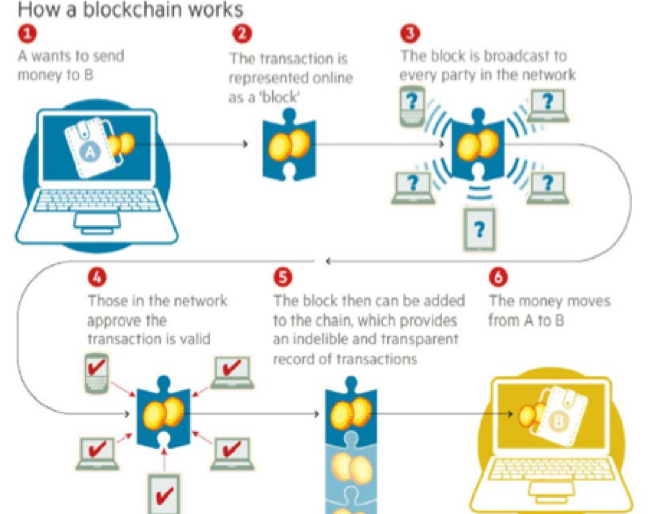
\includegraphics[width=\paperwidth-200]{images/blockchain?}
        \caption{Illustreert hoe de blockchain werkt \cite{howBlockchainWorks}}
        \label{fig:blockchain?}
    \end{center}
\end{figure}
\newpage

In dit onderzoek gebruiken we de beschrijving van het ICTU \footnote{https://www.ictu.nl/}, die de blockchain beschrijft als: een specifieke databasetechnologie die leidt tot een gedistribueerd autonoom grootboeksysteem \cite{kaptijn}. De integriteit van dit gedistribueerd autonoom grootboeksysteem wordt gewaarborgd doordat iedere partij zeggenschap heeft bij de validatie van een transactie. Dit versnelt het proces doordat beheerders en tussenpersonen worden uitgeschakeld. Meningsverschillen worden opgelost door een cryptografisch consensus algoritme (zie paragraaf \ref{cap:consensus}).\par

De blockchain technologie lost verschillende problemen op die voorkomen bij het gebruik van traditionele gecentraliseerde database technologie ̈en die in handen zijn van één instantie. Dit soort technologie ̈en vereisen vertrouwen dat de beheerder zorgvuldig omgaat met de toegang of bewerkingen van de data. Verder dient de database toegankelijk te zijn voor de belanghebbende en dat hij erop kan vertrouwen dat de instantie er de volgende dag nog is. Deze problemen komen niet voor in een gedecentraliseerde blockchain database. Dit komt omdat een nieuwe dienst, softwarebedrijf of markten op de blockchain de volgende zes designprincipes \cite{blockRev} hanteren:
\begin{enumerate}
	\item Netwerk integriteit\\
	Het systeem bewaakt de data integriteit doordat ieder lid in het netwerk alle transacties kan nalopen en kan controleren, in plaats van een enkel lid die dit proces uitvoert. Gebruikers op het netwerk kunnen rechtstreeks waarde met elkaar uitwisselen door dit te registeren op een blok. Elk blok heeft een verwijzing naar een voorgaand blok, waardoor niemand een transactie kan verbergen of kan vervalsen. Dit omdat er meer andere gebruikers zijn met de juiste realiteit.
	\item Gedistribueerd\\
	Het systeem is volledig Gedistribueerd. Dit houdt in dat er geen één punt is van controle of falen. Er is niet een gebruiker of organisatie die het systeem uit kan zetten.
	\item Security\\
	Satoshi’s white paper \cite{bitcoinPaper} vereist dat het systeem beveiligd is door een public key infrastructure (PKI) \footnote{https://en.wikipedia.org/wiki/Public\_key\_infrastructure}. De PKI is een geavanceerde vorm van asymmetrische cryptografie, waar de gebruiker zowel een publiek en privé sleutel ontvangt om zichzelf binnen het netwerk te identificeren en berichten kan versleutelen en ontsleutelen.
	\item Eigendomsrechten\\
	Eigendomsrechten over valuta en andere data zijn transparant in het netwerk en dus beschikbaar voor iedere gebruiker van het netwerk. Hierdoor dient een blockchain als een publiek register door middel van een tool genaamd Proof of Existence (PoE) \footnote{https://en.wikipedia.org/wiki/Proof\_of\_Existence}. Deze tool creëert en registreert de cryptografische overzichten van akten, licenties en andere rechten van gebruikers.
	\item Privacy\\
	Gebruikers beheren hun eigen data. Er is geen centrale partij en gebruikers op het netwerk geven zelf aan wat ze aan informatie vrijgeven. Dit is echter allemaal optioneel en een gebruiker op de blockchain hoeft in de meeste implementaties alleen een publieke en private key te hebben. De gehele identificatie- en verificatie laag zijn los van elkaar waardoor gebruikers op de blockchain de mogelijkheid hebben om anoniem te zijn.
	\item Valuta als motivatie\\
	Het systeem motiveert deelnemers van het netwerk door ze valuta te geven voor bepaalde acties op het netwerk. In het geval van de bitcoin, krijgen miners bitcoin geld voor het eerstvolgende blok te koppelen aan het vorige blok aan data. Dit wordt gedaan door een cryptografische puzzel op te lossen die geleidelijk lastiger wordt.
\end{enumerate}
\newpage

\section{Type Blockchain}
Om een geïnformeerd besluit te maken welk type blockchain juist is voor het proof of concept worden de verschillende type blockchain in dit paragraaf behandeld. Dit wordt gedaan vanaf een hoog technisch niveau. In essentie zijn er drie types blockchain: privé, consortium en openbaar. Deze types kunnen daarna weer onderverdeeld worden in de open en gesloten categorieeën blockchain. Per type blockchain wordt er ook gelijk gekeken naar de grote projecten die relevant zijn. Zodat in een vervolg hoofdstuk hierover een vergelijking kan worden uitgevoerd.\par
					
De categorie gesloten, waarin de types privé en consortium zitten zijn bedoeld voor een gelimiteerde omgeving zoals één of meerdere bedrijven en organisaties. Terwijl een openbare blockchain volledig open is en geen permissies zijn die mensen of systemen erbuiten houden.

\subsection{Privé Blockchain}
Voor een volledige private blockchain, moeten de schrijfrechten op een centrale plek staan die beheerd worden door een organisatie. De leesrechten kunnen zowel publiekelijk of ook net zo beperkt zijn als de schrijfrechten. Applicaties die gebruik maken van een privé Blockchain zijn interne applicaties die alleen gebruikt worden binnen een bedrijf of organisatie. Want in andere gevallen wordt publieke leesrechten en controleerbaarheid vereist \cite{privateBlockChains}. Voorbeelden van privé Blockchains zijn MultiChain en Hyperledger:\par
\textbf{MultiChain} - MultiChain is een platform voor het ontwikkelen en publiceren van privé blockchains. Het lost een aantal schaalbaarheid problemen \cite{oreillyScalability} van de blockchain op met een geïntegreerde gebruiker permissie systeem. Verder biedt het bedrijven de mogelijkheid om zonder software ontwikkelaars een blockchain op te richten \cite{mutlichain}.

\textbf{Hyperledger} - Hyperledger is een open source project. Het wordt ontwikkeld met als doel om een geavanceerd bedrijfstak overkoepelende blockchain implementatie te realiseren. Het wordt ondersteund door de Linux Foundation \cite{linuxFoundation} en wordt gezamenlijk ontwikkeld door grote organisatie in financiën, banken, IoT, productie en technologie \cite{hyperledger}.

\subsection{Consortium Blockchain}
Het consortium blockchain type is gedeeltelijk privé. Het onderscheidt zich in het consensus (zie paragraaf \ref{cap:consensus}) proces waar alleen een aantal vooraf geselecteerde peers (gebruikers) de integriteit van de data op de blockchain waarborgen. Deze nodes zijn bijvoorbeeld 10 grote financi ̈ele instellingen die bij de aanmaak van een nieuwe block aan de blockchain zeggenschap hebben. Andere deelnemers van de blockchain hebben nog steeds het recht om de besluiten van de 10 nodes te controleren, maar ze hebben verder geen stem over het feit of de volgende block valide is.\par
\newpage					
Het voordeel van de consortium variant is dat deze efficiënter is en toch voldoende transactie transparantie geeft. Ook is het niet een bedrijf die alleen oordeelt over de data. Voorbeelden van dit type zijn Ethereum en R3:

\textbf{Ethereum} - Het Ethereum project beschrijft zichzelf als een gecentraliseerd platform voor applicaties die precies uitgevoerd worden zoals ze geprogrammeerd zijn. Dit allemaal zonder enige kans van fraude, censuur of veranderingen van derden \footnote{https://www.ethereum.org/}. Applicaties, smart contracts, worden geprogrammeerd in de Solidity taal die voor het Ethereum project is ontwikkeld. Het wordt open-source ontwikkeld en er is een bondgenootschap, de Enterprise Ethereum Alliance\footnote{https://entethalliance.org/} dat bestaat uit 315 fortune 500 bedrijven en organisaties, die gezamenlijk werken aan het het enige platform die smart contracts ondersteunt op de blockchain.\cite{ethWood}\par

Het project kan gezien worden als een verder uitgewerkte versie van Bitcoin die meer functionaliteiten toevoegt. Zo bestaat de status van Ethereum netwerk net zoals de Bitcoin uit meerdere objecten die 'accounts' worden genoemd, waarbij elk account een adres van 20 bytes en statusovergangen heeft. De staat van deze objecten worden opgeslagen in de blockchain waaruit gelijk afgeleid kan worden waar valuta naartoe gaat.\cite{whitePaperEthereum}

\textbf{R3} - Dit is een gedistribueerd database-technologiebedrijf in New York. Het is verbonden met veel van ’s werelds grootste financiële instellingen, met als missie om de voordelen van de blockchain te realiseren. Het is momenteel nog enorm in ontwikkeling en het bedrijf voert vooral onderzoek uit\cite{R3}.

\subsection{Openbare Blockchain}
Dit type blockchain is zoals de naam al aangeeft publiek beschikbaar tot iedereen in de wereld. Dit houdt in tegenstelling tot Consortium ook het consensus (zie paragraaf \ref{cap:consensus}) proces in. Iedere gebruiker op het netwerk is gelijk en heeft zeggenschap op de geldigheid van nieuwe data blokken.\par

Een volledig publieke blockchain is een open-source systeem die gebruikers met economisch doeleinde motiveert om samen te werken. Dit principe heet crypto economics en hierdoor kunnen ontwikkelaars belangen zoals beschikbaarheid waarborgen. Zo zal een transactie met een hoger tarief resulteren in snellere conversie. Een voorbeeld hiervan is het bekende Bitcoin project.

\textbf{Bitcoin}. Bitcoin is het bekendste voorbeeld van een blockchain project. Bitcoin staat vooral bekend als digitale valuta en online betalingssysteem die door gebruik van cryptografie om valuta-eenheden te geneert en reguleert. Verder gebruikt het cryptografie om de overdracht van fondsen te verifiëren zonder een centrale bank.\par